\chapter{Implementasjon}

Følgende avsnitt beskrive hva som er implementert av de ting som er nevnt i oppgaveteksten og som ekstra ting i applikasjonen. 

\section{Fragment}
Det benyttes fragmenter fremst in listen for alle kontakter som er presentert i figur \ref{fig:liste_fragment}, side \pageref{fig:liste_fragment}. Listefragmentet bruker en egen layout fil i to versjon for liggende og stående orientering.
Andre fragmenter som også benyttes er dialog fragment i form av en bekreftelse ved lagring eller endring av en kontakt. 
Det siste fragmentet som brukes er preferance fragment der det brukes standard oppsett av en preferance liste som finnes i systemet (figur \ref{fig:preferance_fragment}, side \pageref{fig:preferance_fragment}. 
Alle instillinger som blir endret via preference fragmet blir lagret og lest fra \textit{sharedpreferences}.

\section{Inputvalidering}
Det blir validert input for navn og telefonnummer. Navn blir validert slik at feltet kan ikke være tomt og får kun innholde bokstaver. 
Feltet for telefonnummer blir validert med to regex strenger, en som tester på at det er kun tall som brukes og det andre om at lengden på tallrekken får være mellom 8 og 12 tall. Se figur \ref{fig:validering}, side \ref{fig:validering}.

\section{Database}
Det benyttes en sqlite databse med kolonner som motsvarer alle de felt som finnes i Person objektet. Disse er id, navn, melding til personen, dato for bursdag, tid for individuell utsendelse av melding (benyttes ikke), erAktiv (dersom man ønsker at meslding service skal være aktiv eller ikke til den personen). Person objekter oprettes fra databasen gjennom vanlige sql spørringer. Detsamme gjelder også for lagring. 


\section{Services og Broadcas receiver}
I applikasjonen brukes det totalt to servicer og en broadcast receiver som kaller opp første hovedservicen etter oppstart av telefonen. Dette medfører at applikasjonen trenger ikke startes uten service kommer til å starte automatisk ved systemstart. Hovedservicen kjører hele tiden og ved valgt klokkeslett starter den en sekundær service som ser etter hvilke kontakter i databsen som har bursdag under den aktuelle dagen. Dersom slike personer finnes blir det sendt meldinger med den forhåndsdefinerte teksten. 
Når hoverservicen kjører vises det en nofifikasjon i telefonens info felt (se figur \ref{fig:notification}, side \pageref{fig:notification}9.

\section{Content provider}
Content privider er implementert slik at data som tilhører \texttt{Birthday-o-Matic} er tilgjengelig til andre applikasjoner i systemet. Content provideren er bygget opp gjennom at man benytter seg av direkte spørringer som returnerer collections med person objekter i \texttt{DBHandler} klassen. Sammen med prosjektet er det også levert inn en testapplikasjon som gjør det mulig å teste denne funksjonen (se figur \ref{fig:content_provider}).

\begin{figure}[ht]
    \centering
    \begin{subfigure}[b]{0.35\textwidth}
        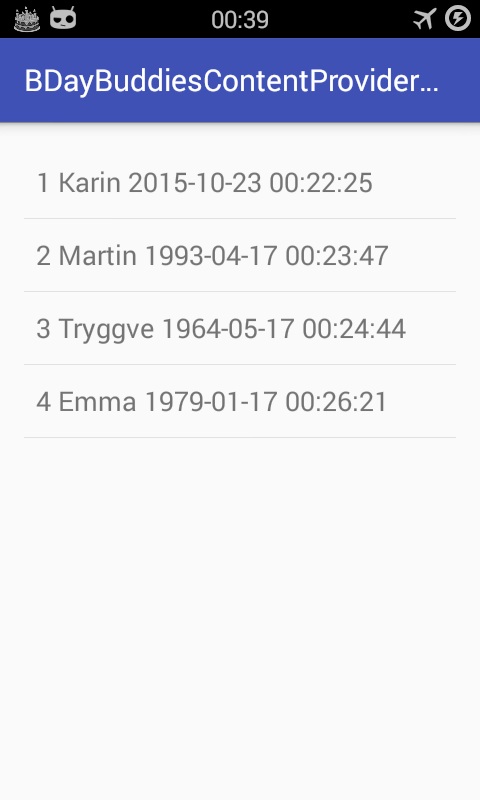
\includegraphics[width=\textwidth]{./img/11.png}
        \caption{Testapp for ContentProvider}
        \label{fig:test_content_provider}
    \end{subfigure}
    \begin{subfigure}[b]{0.35\textwidth}
        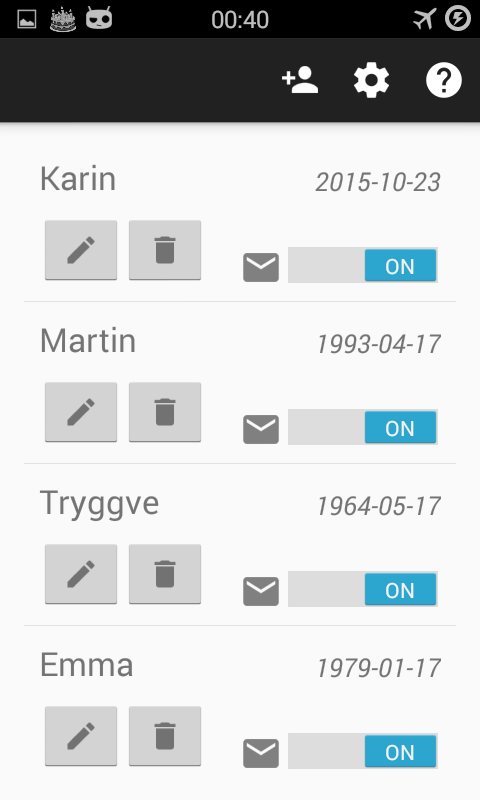
\includegraphics[width=\textwidth]{./img/12.png}
        \caption{Gjenspeiler data i hovedappen}
        \label{fig:test_hovedapp}
    \end{subfigure}
    \caption{Demo av ContentProvider}
    \label{fig:content_provider}
\end{figure}




\chapter{Aktiviteter}
Kapitelet viser en oversikt over alle aktiviteter i applikasjoner. Ved oppbyggingen av de grafiske komponentene i applikasjonen har jeg valgt å fokusere på å tinærme seg så godt som mulig en \textit{native} applikasjon gjennom å direkte modifisere standard komponenter uten noen overdriven fargetema eller custom fonter. Tanken er at brukeren skal kjenne seg så mye som mulig fra en standard kontakt applikasjon som man ofte bruker på telefonen. Denne bursags appen kommer ikke til å benyttes ofte med brukergrensesnitt ettersom etter man har registrert alle ønskelige kontakter kommer brukeren mest sannsynelig ikke å ha noen frekvent interaksjon med applikasjoenen. Derfor er det fremst lag tfokus på at brukeren skal direkte kjenne igjenn hvorda man bruker applikasjonen, også dersom det har gått lang tid mellom de ganger som applikasjonen brukes. I dette kapitel presenteres derfor bilder av de viktigste aktivitetetne og UIX komponetner som er opprettet for applikasjonen. 

\begin{figure}[ht]
    \centering
    \begin{subfigure}[b]{0.35\textwidth}
        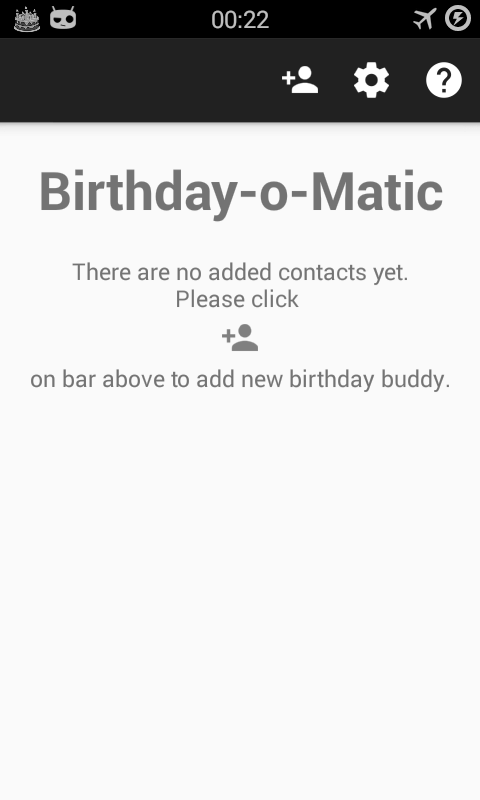
\includegraphics[width=\textwidth]{./img/1.png}
        \caption{Ingen kontakter registrert}
        \label{fig:ingen_kontakter}
    \end{subfigure}
    \begin{subfigure}[b]{0.35\textwidth}
        
\includegraphics[width=\textwidth]{./img/2.png}
        \caption{Ny kontakt}
        \label{fig:ny_kontakt}
    \end{subfigure}
    \begin{subfigure}[b]{0.35\textwidth}
        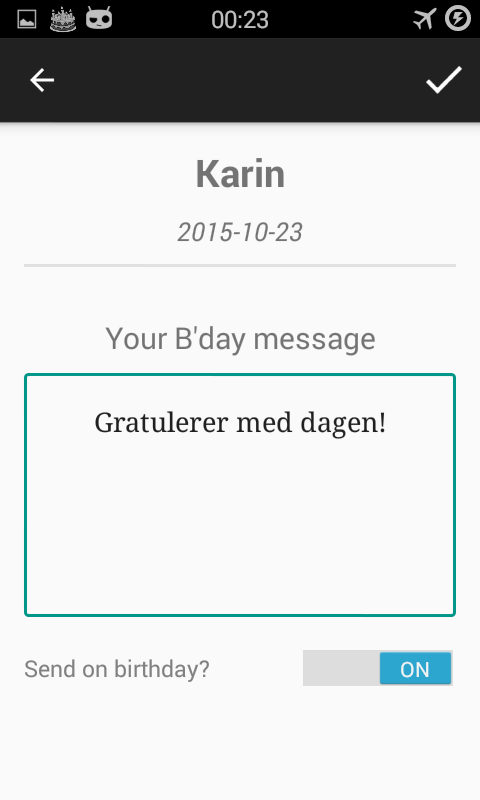
\includegraphics[width=\textwidth]{./img/3.png}
        \caption{Melding}
        \label{fig:melding}
    \end{subfigure}
    \begin{subfigure}[b]{0.35\textwidth}
        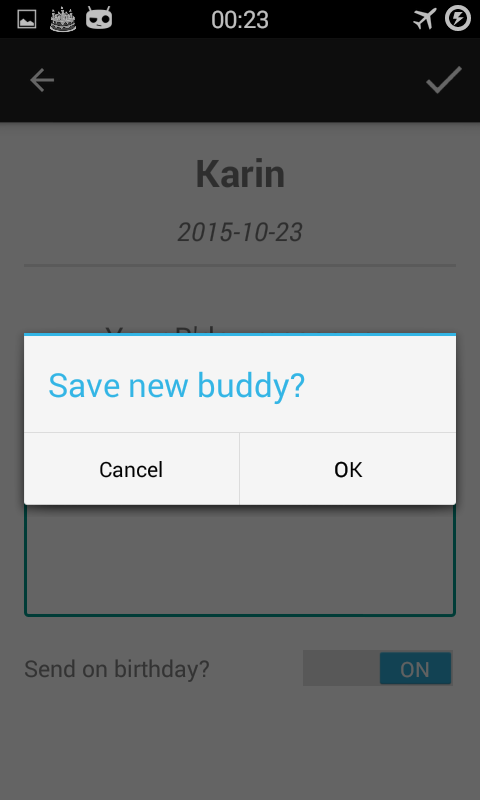
\includegraphics[width=\textwidth]{./img/4.png}
        \caption{Dialog fragment}
        \label{fig:dialog_fragment}
    \end{subfigure}
    \caption{Fremgang for å legge til en ny kontakt.}
    \label{fig:ny_kontakt_workflow}
\end{figure}


\begin{figure}[ht]
    \centering
    \begin{subfigure}[b]{0.35\textwidth}
        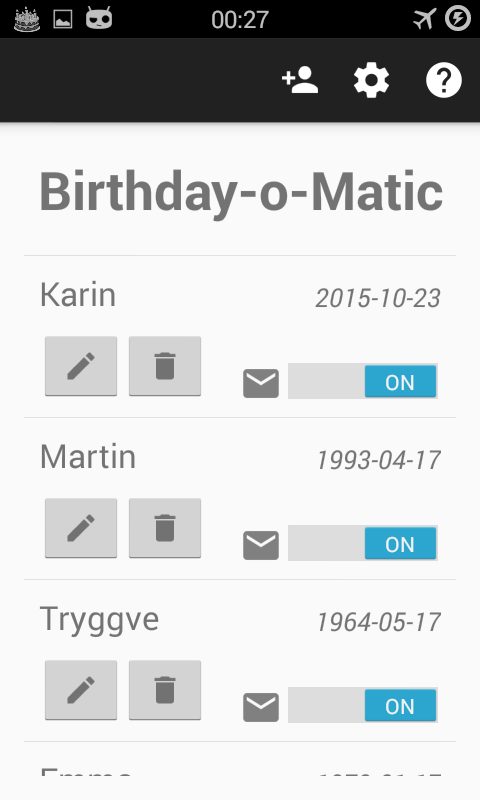
\includegraphics[width=\textwidth]{./img/5.png}
        \caption{Liste fragment (portrait)}
        \label{fig:liste_fragment_p}
    \end{subfigure}
    \begin{subfigure}[b]{0.6\textwidth}
        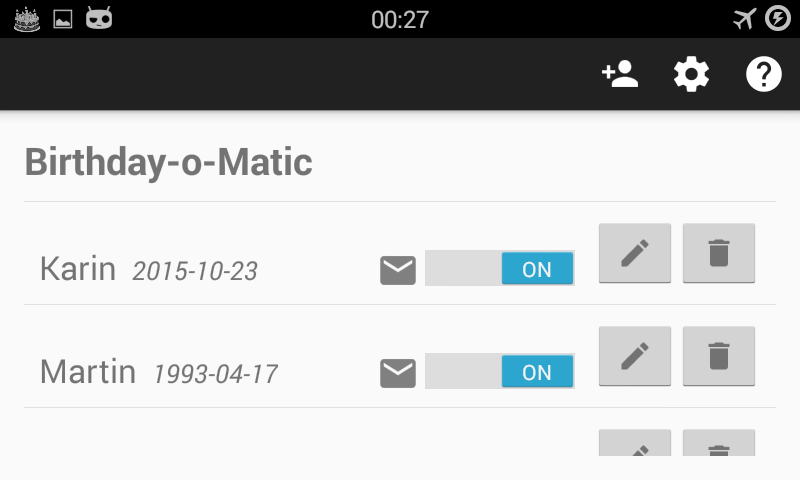
\includegraphics[width=\textwidth]{./img/6.png}
        \caption{Liste fragment (landscape)}
        \label{fig:liste_fragment_l}
    \end{subfigure}
    \caption{Varierende orientering av liste fragment}
    \label{fig:liste_fragment}
\end{figure}


\begin{figure}[ht]
    \centering
    \begin{subfigure}[b]{0.35\textwidth}
        
\includegraphics[width=\textwidth]{./img/2.png}
        \caption{Ny kontakt (portrait)}
        \label{fig:ny_kontakt_p}
    \end{subfigure}
    \begin{subfigure}[b]{0.6\textwidth}
        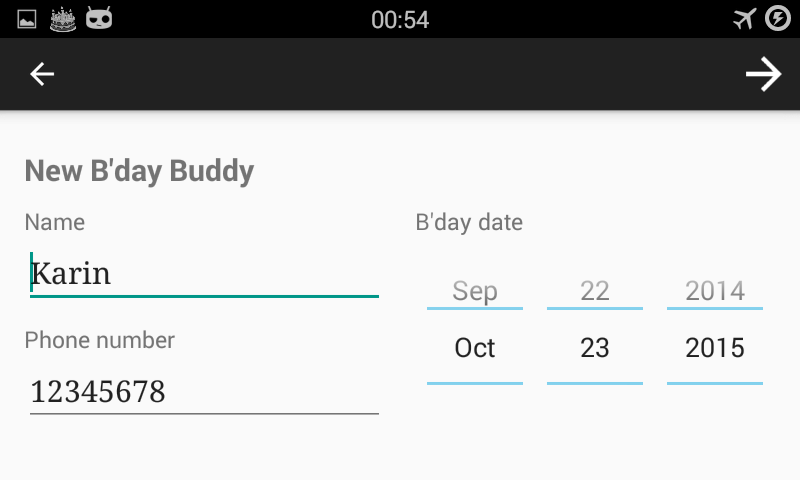
\includegraphics[width=\textwidth]{./img/13.png}
        \caption{Ny kontakt (landscape)}
        \label{fig:ny_kontakt_l}
    \end{subfigure}
    \caption{Orientering av ny kontakt aktivitet}
    \label{fig:ny_kontakt_aktivitet}
\end{figure}

\begin{figure}[ht]
    \centering
    \begin{subfigure}[b]{0.35\textwidth}
        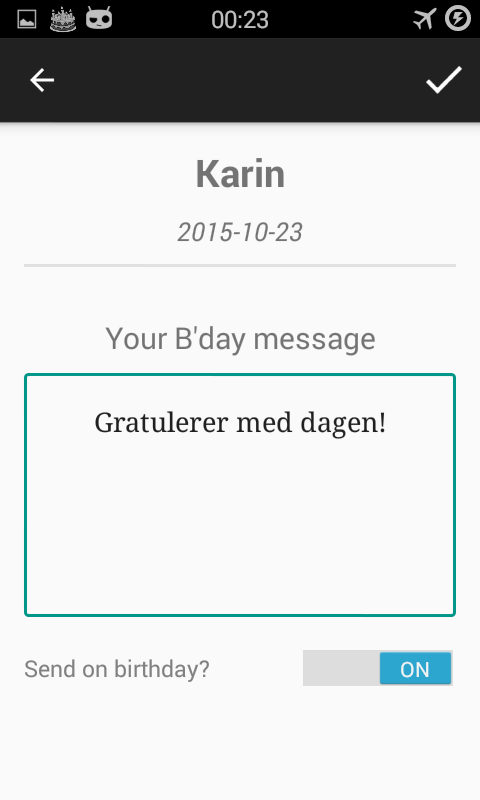
\includegraphics[width=\textwidth]{./img/3.png}
        \caption{Melding (portrait)}
        \label{fig:melding_p}
    \end{subfigure}
    \begin{subfigure}[b]{0.6\textwidth}
        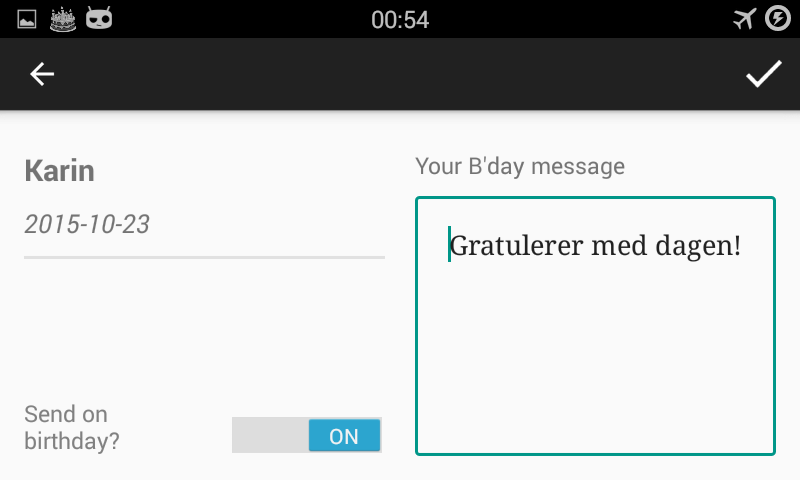
\includegraphics[width=\textwidth]{./img/14.png}
        \caption{Melding (landscape)}
        \label{fig:melding_l}
    \end{subfigure}
    \caption{Orientering av melding aktivitet}
    \label{fig:melding_aktivitet}
\end{figure}

\begin{figure}[ht]
    \centering
    \begin{subfigure}[b]{0.35\textwidth}
        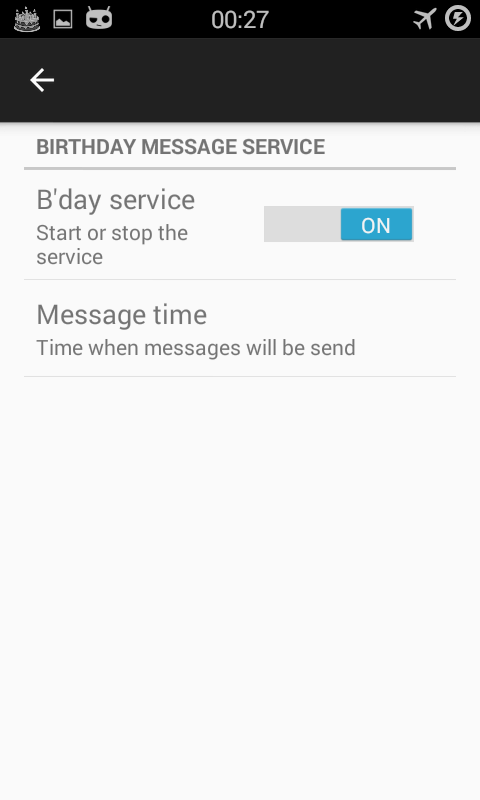
\includegraphics[width=\textwidth]{./img/7.png}
        \caption{Preference fragment}
        \label{fig:preferance_fragment}
    \end{subfigure}
    \begin{subfigure}[b]{0.35\textwidth}
        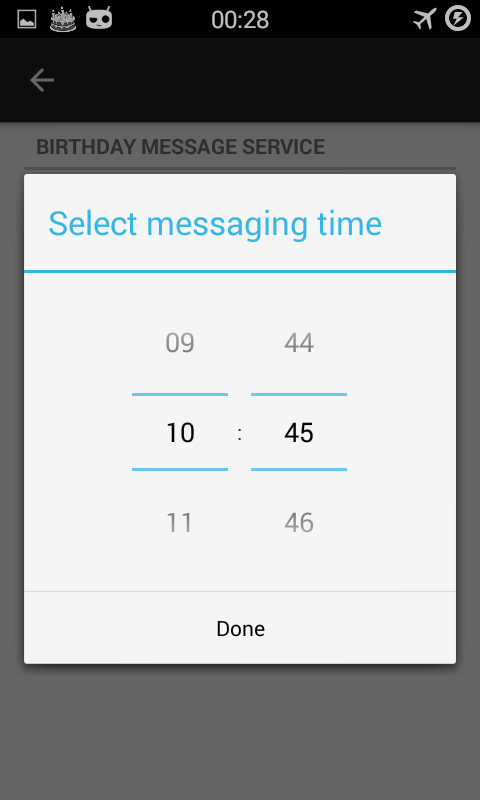
\includegraphics[width=\textwidth]{./img/8.png}
        \caption{Tid for seding}
        \label{fig:melding_tid}
    \end{subfigure}
    \begin{subfigure}[b]{0.35\textwidth}
        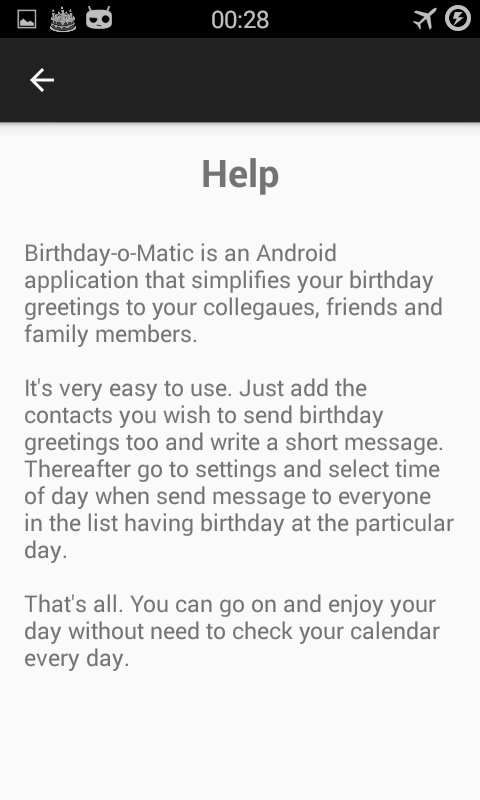
\includegraphics[width=\textwidth]{./img/9.png}
        \caption{Hjelp aktivitet}
        \label{fig:hjelp_aktivitet}
    \end{subfigure}
    \begin{subfigure}[b]{0.35\textwidth}
        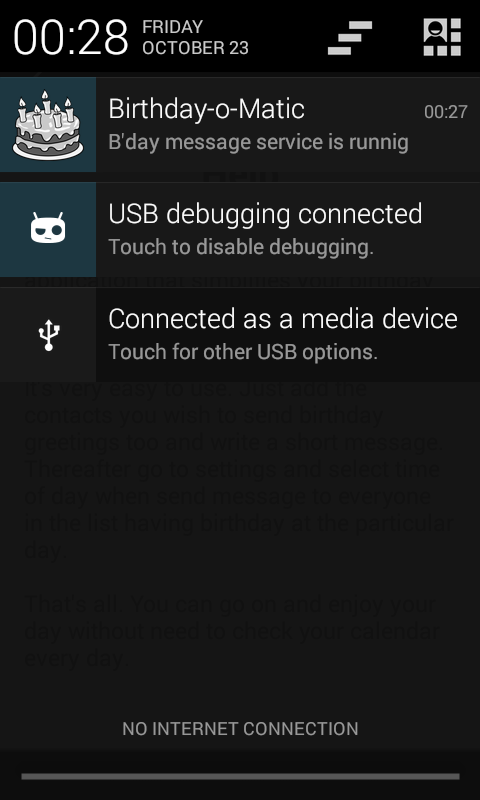
\includegraphics[width=\textwidth]{./img/10.png}
        \caption{Service notification}
        \label{fig:notification}
    \end{subfigure}
    \caption{Øvrige aktiviteter og fragmenter.}
    \label{fig:ovrige_aktiviteter}
\end{figure}

\begin{figure}[ht]
    \centering
    \begin{subfigure}[b]{0.35\textwidth}
        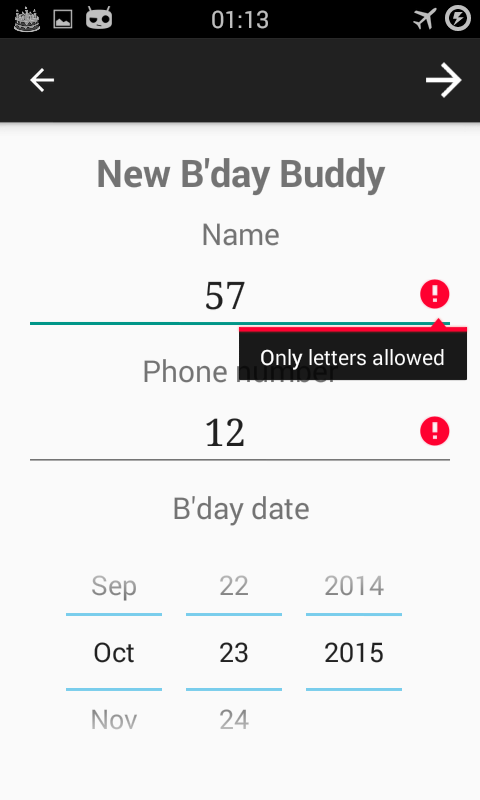
\includegraphics[width=\textwidth]{./img/15.png}
        \caption{Validering av navn}
        \label{fig:validering_tekst}
    \end{subfigure}
    \begin{subfigure}[b]{0.35\textwidth}
        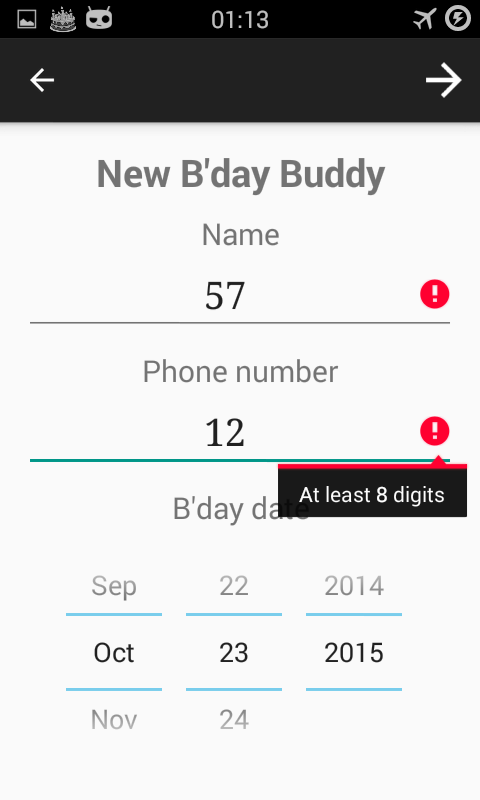
\includegraphics[width=\textwidth]{./img/16.png}
        \caption{Validering av telefonnummer}
        \label{fig:validering_tall}
    \end{subfigure}
    \caption{Inputvalidering}
    \label{fig:validering}
\end{figure}


\chapter{Veien videre}
Føgende avsnitt beskriver noen funksjonalitet og forbedringer som jeg ønsker at skal implementeres under videre utvikling av applikasjoenen. 

\begin{description}
\item[Varsler]
I informasjons feltet for telefonen bør det bli vist en melding etter at man har sendt ut meldinger til en person. Dette kan være greit for brukeren som en enkel påminnelse om at hilsen er blitt sendt.

\item[Tidssoner]
Det hadde vært fint å ha mulighet til å spesifisere andre tidssoner for kontaktene slik at man ikke sender melding til noen mindt på natten.

\item[Valideringslytter]
Nå blir inputsvalidering kjørt samtidig som brukeren klikker på videre knappen. En eventuell forbedring kan være at man validerer så snart et felt har mistet fokus. Slik funksjonalittet vil gi brukeren hyppigere respons på feil input. 

\item[Meldings kontroll]
En overordnet struktur som kvalitetssikrer at servicen ikke sender melding til en person to ganger samme dag dersom servicen blir startet om. Dersom man starter om hovedservice f.eks. ved om start av telefonen kommer hovedservice å kjøre dersom tiden for utsendelse er satt tilbake i tid. Dette gjøres ettersom systemet forsøker kjøre servicen dersom systemet tror at servicen ikke har kjørt. Slik funksjonalitet er helt riktig slik at man ikke misser å sende melding en dag også når telefonen blir skrudd av under den planlagdte tiden for sending av meldinger. Det som mangler er at man setter en enkel flagg feks i databasen eller delte innstillinger den første gangen meldingen blir sendt sammen dag.


\item[Custom datepicker]
DAtepickeren som brukes nå er begrenset slik at man ikke kan sette dato i fremtiden. Det som kanskje hadde væert med funksjonelt er en data picker som tilbyr kun dag å månded ettersom egentlig er det ikke egentligen nødvendig å registrer fødseldag for kontaktene uten det eneste som vi trenger er dag og måned.

\item[Historikk]
En enkel form av historikk for hvikle personer som man har sendt meldinger til. 

\item[Import]
Det er flere applikasjoner på telefonen som har en egen content provider og kan f.eks. brukes til å velge kontakter som man ønsker å importere fra telefonens kontaktliste eller apper for sosiale medier.

\end{description}


